\documentclass{article}[12pt]

\usepackage[utf8]{inputenc}
\usepackage{amsmath}
\usepackage{graphicx}
\usepackage{subcaption}
\usepackage{float}
\usepackage[a4paper, margin=1in]{geometry}
\usepackage{hyperref}

\graphicspath{./images/}

\title{Création d'une plateforme pour l'analyse du signal posturographique \\
\textbf{Troisième semaine}}
\author{Inès PINGAULT, Anaëlle MAZOUNI, Hippolyte DEPARIS \\
Lille }

\date{\today}

\begin{document}
\maketitle

\newpage
\tableofcontents

\newpage
\section{Introduction}

La posturographie, aussi appelée posturologie, est une technique employée pour évaluer, 
mesurer et contrôler la posture en position debout. Pour maintenir un équilibre vertical, 
le corps humain ajuste en permanence sa posture par rapport à son environnement en fonction de 
certains signaux qu'il reçoit. Ces signaux sont captés par les yeux, la colonne vertébrale, 
l’oreille interne ou encore les pieds. Le cerveau les analyse et envoie des instructions au 
corps dans le but de modifier sa posture en temps réel aux différents éléments perçus. Si ces 
signaux, importants pour le maintien de l'équilibre ne sont pas ou mal perçus, ou mal analysés,
la posture ne sera pas correctement adaptée, et des troubles tels que des déséquilibres, des 
vertiges ou encore des problèmes musculosquelettiques pouvant aller jusqu'à des douleurs 
chroniques dans certaines régions de l’organisme pourraient apparaître. Il est donc important 
pour les posturologues de mettre aujourd’hui l’accent sur l'étude du rôle des yeux, des pieds 
ainsi que les occlusions dentaires dans les problèmes liés à la posture. Cette discipline étudie
la position de l’homme dans l’espace (son équilibre, sa stature, son aplomb, sa stabilité...)
grâce à des appareils de mesure spécialisés. Elle prend en compte la capacité de rester en 
équilibre sur ses pieds ainsi que la symétrie du corps ou la perception visuelle de 
l'horizontalité. Ces études sont possibles aussi bien dans des situations statiques que 
dynamiques. La posturographie dynamique informatisée (non étudiée dans ce rapport) est une 
technique d’évaluation clinique non invasive permettant de quantifier les mécanismes
d’adaptation du système nerveux central lorsque le corps est en mouvement (Figure 1).  
La posturographie statique évalue quant à elle la posture d’un patient en équilibre
orthostatique (position érigée immobile, fondamentale de l'espèce humaine). Cette évaluation
se fait en positionnant debout, le patient sur une plateforme équipée de nombreux capteurs 
de pression. L’enregistrement des oscillations du centre de pression des pieds permettent 
de retracer l'évolution du centre de gravité (ou centre de masse) du patient. Lors de ces 
évaluations, on étudie aussi la réponse posturale du patient à certaines perturbations 
(Figure 2).


\begin{figure}[ht]
    \centering
    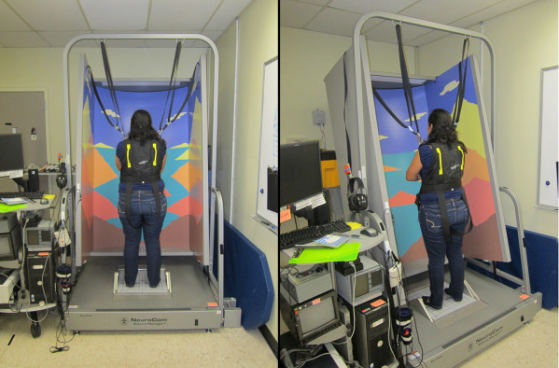
\includegraphics[width=0.5\textwidth]{images/introduction/dynamique.png}
    \caption{Machine d’analyse de la posturographie dynamique }
    \label{fig:posturographie-dynamique}
\end{figure}

\begin{figure}[ht]
    \centering
    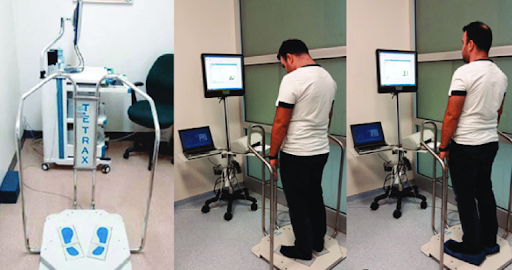
\includegraphics[width=0.5\textwidth]{images/introduction/statique.png}
    \caption{Machine d’analyse de la posturographie statique }
    \label{fig:posturographie-statique}
\end{figure}



\newpage
% \section{Signal analysé en posturographie statique}

\subsection{Pression plantaire}

Les pressions plantaires mesurent la répartition des forces sous les pieds au niveau des zones d’appui.
Ces pressions sont capturées par des capteurs disposés sur une surface ou intégrées dans des semelles.
Ces mesures permettent d’identifier les points de pression maximale et minimale, fournissant des données sur la statique et la dynamique du pied.
Les centres de pression sont calculés à partir des variations de pression.
Ils reflètent les ajustements dynamiques de la posture en réponse aux déséquilibres.
Les mesures de ces signaux nous permettent de cartographier les zones d'appui et de visualiser les charges appliquées sur les pieds.
On peut alors identifier les zones à risque de pathologie (comme l’hallux valgus ou la fasciite plantaire).
L'évaluation des déséquilibres ou anomalies dans la distribution des forces est alors possible.
Les études sont appliquées en podologie et orthopédie, pour détecter les troubles plantaires ou les anomalies posturales.
Elles sont aussi utilisées pour suivre les progrès post-blessures ou post-chirurgie de patients.
Enfin, on peut aussi les mener dans le but d’optimiser les performances athlétiques en analysant les impacts au sol.

\subsection{Méthode d'enregistrement}

Les plateformes stabilométriques mettent l’accent sur l'étude des mouvements posturaux en évaluant les forces verticales et les déplacements dans les plans horizontal et vertical.
Ces plateformes disposent fréquemment d’instruments additionnels, comme des surfaces instables ou des systèmes de visualisation interactifs pour perturber l'équilibre et examiner les réactions compensatoires du patient.
Ces dispositifs sont utilisés pour évaluer la stabilité posturale en position debout, notamment chez des patients atteints de troubles neurologiques ou vestibulaires.
Ils sont également utilisés pour détecter les déficiences proprioceptives et pour la rééducation.
En gériatrie, ils permettent d'évaluer les risques de chute, et en sport, ils servent à optimiser les stratégies d' équilibre.\\

\textbf{Exemples :}
\begin{itemize}
  \item Stabilo Stabilometric Platform
  \item Plateforme Satel
\end{itemize}

\begin{figure}[H]
 \centering
  \begin{subfigure}[b]{0.45\textwidth}
    \centering
    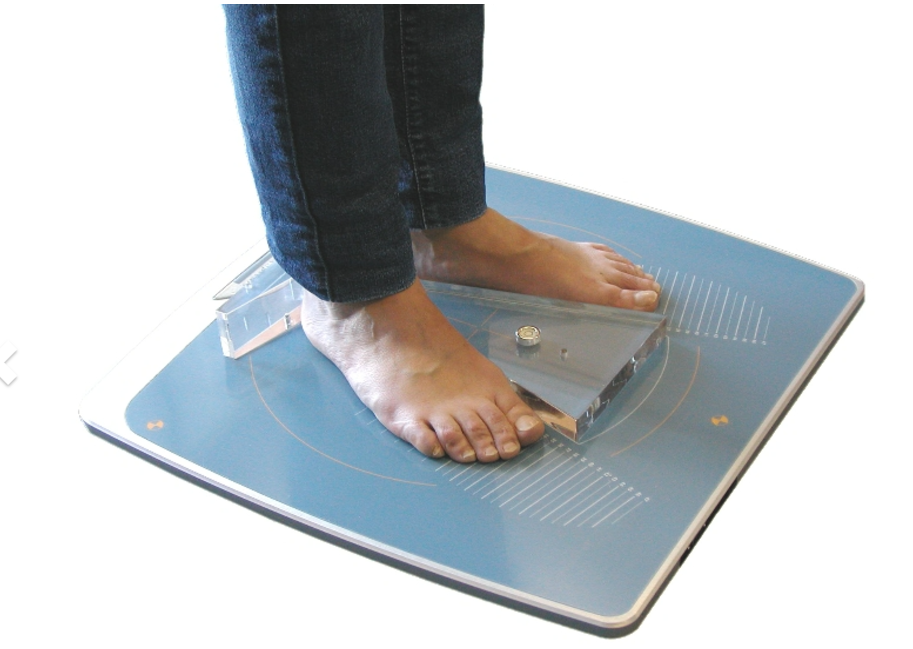
\includegraphics[height=5cm]{images/pression_plantaire/plateforme-stabilometrique.png}
    \caption{Plateforme stabilométrique}\label{fig:plateforme_stabilometrique}
  \end{subfigure}
  \begin{subfigure}[b]{0.45\textwidth}
   \centering
    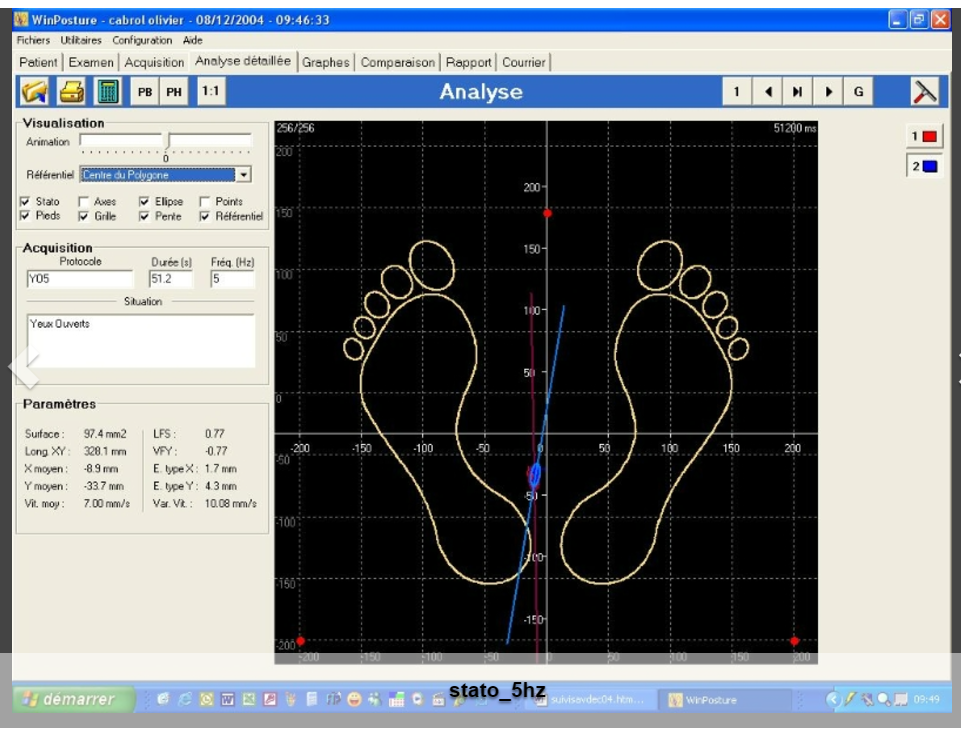
\includegraphics[height=5cm]{images/pression_plantaire/winposture.png}
    \caption{Logiciel de visualisation Winposture}\label{fig:winposture}
  \end{subfigure} \\
  \begin{subfigure}[b]{0.45\textwidth}
    \hspace{-1.5cm}
    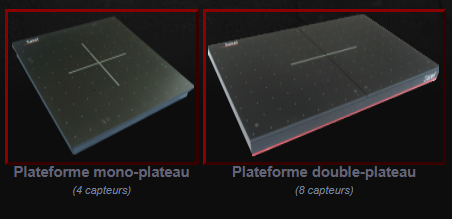
\includegraphics[height=5cm]{images/pression_plantaire/satel.png}
    \caption{Plateforme stabilométrique Satel}\label{fig:satel}
  \end{subfigure}
  % \caption{Ill}\label{fig:exemple_plateforme_force}
\end{figure}

\begin{figure}[ht]
  \centering
  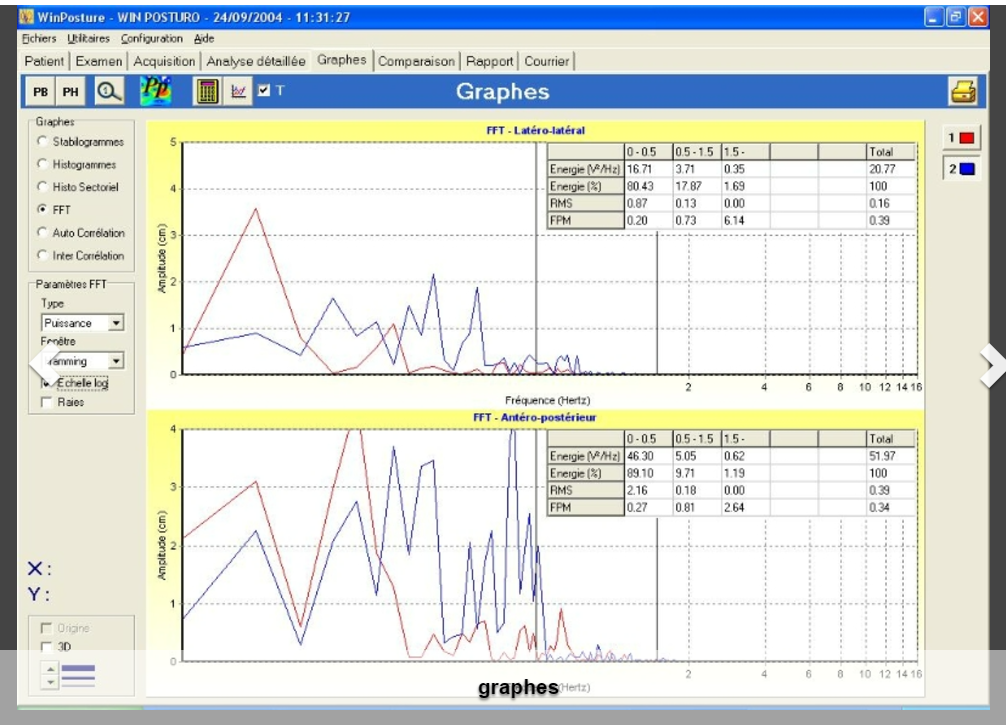
\includegraphics[height=10cm]{images/pression_plantaire/winposture2.png}
  \caption{Logiciel Winposture}\label{fig:winposture2}
\end{figure}

\section{Signaux de posturographie statique}

\subsection{Signaux étudiés}

\subsubsection{Types de signaux}
Les pressions plantaires mesurent la répartition des forces sous les pieds au 
niveau des zones d’appui. Ces pressions sont capturées par des capteurs disposés 
sur une surface ou intégrées dans des semelles. Ces mesures permettent 
d’identifier les points de pression maximale et minimale, fournissant des données 
sur la statique et la dynamique du pied. Les centres de pression sont calculés à 
partir des variations de pression. Ils reflètent les ajustements dynamiques de la 
posture en réponse aux déséquilibres. Les mesures de ces signaux nous permettent 
de cartographier les zones d'appui et de visualiser les charges appliquées sur les
pieds. On peut alors identifier les zones à risque de pathologie (comme l’hallux 
valgus ou la fasciite plantaire). L'évaluation des déséquilibres ou anomalies dans 
la distribution des forces est alors possible. Ces études sont appliquées en 
podologie et orthopédie, pour détecter les troubles plantaires ou les anomalies 
posturales. Elles sont aussi utilisées pour suivre les progrès post-blessures ou 
post-chirurgie de patients. Enfin, on peut aussi les mener dans le but d’optimiser 
les performances athlétiques en analysant les impacts au sol.

\subsubsection{Enregistrement des signaux}
Les plateformes stabilométriques, a l’instar des plateformes de force, mettent 
particulièrement l’accent sur l'étude des mouvements posturaux en évaluant les 
forces verticales et les déplacements dans les plans horizontal et vertical. Ces 
plateformes disposent fréquemment d’instruments additionnels, tels que des surfaces 
instables ou des systèmes de visualisation interactifs, pour perturber l'équilibre 
et examiner les réactions compensatoires du patient. Ces dispositifs sont utilisés 
pour évaluer la stabilité posturale en position debout, notamment chez des patients 
atteints de troubles neurologiques ou vestibulaires. Ils sont également utilisés 
pour détecter les déficiences proprioceptives et pour la rééducation. En gériatrie, 
ils permettent d'évaluer les risques de chute, et en sport, ils servent à optimiser 
les stratégies d' équilibre.\\ 

Exemples : 
\begin{itemize}
    
    \item Stabilo Stabilometric Platform 
    \item Plateforme  Satel (Figure 3)
\end{itemize}

\begin{figure}[ht]
    \centering
    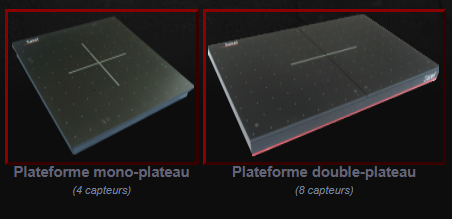
\includegraphics[height=5cm]{images/pression_plantaire/satel.png}
    \caption{Plateforme stabilométrique Satel}\label{fig:satel}
\end{figure}

\subsubsection{Examens cliniques}

L’équilibre postural d’un patient repose entièrement sur le bon fonctionnement de 
son système postural. De légères perturbations ou dérèglements du fonctionnement 
de ce système postural peuvent  entraîner un déséquilibre. Ainsi, les examens 
cliniques de l’équilibre statique sont primordiaux pour détecter de potentielles 
perturbations et éviter par la suite des problèmes de chute.  Parmi ces nombreux 
examens (détaillés en annexe), certains sont fréquemment utilisés : Le Romberg 
postural (Figure 4(a)) , le test de piétinement de Fukuda (Figure 4(b)) ou encore 
d’autres alternatives (Figure 4(c)). 


\begin{figure}[ht]
    \centering
    \begin{subfigure}[b]{0.45\textwidth}
      \centering
      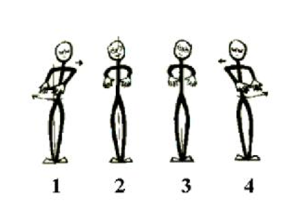
\includegraphics[height=5cm]{images/Exam_cli/Romberg.png}
    \caption{Test de Romberg postural}\label{fig:Romberg}
    \end{subfigure}
    \begin{subfigure}[b]{0.45\textwidth}
      \centering
      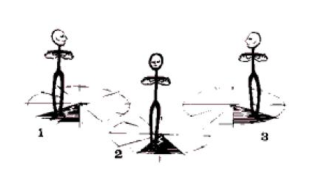
\includegraphics[height=5cm]{images/Exam_cli/pietinement.png}
      \caption{Test de piétinement de Fukuda }\label{fig:pietinement}
    \end{subfigure}
    \begin{subfigure}[b]{0.45\textwidth}
      \centering
      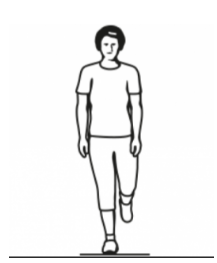
\includegraphics[height=5cm]{images/Exam_cli/Unipodal.png}
    \caption{Test de piétinement de Fukuda }\label{fig:unipodal}
    \end{subfigure}
    \caption{Examens cliniques}\label{fig:global}
  \end{figure}
\subsection{Méthodes d'analyses}

\subsection{Analyse du marché}

Cette analyse de marché a pour objectif de présenter les différentes 
plateformes d'analyse de stabilométrie, en mettant en avant leurs spécificités et 
fonctionnalités, afin d’identifier et répondre aux besoins des professionnels de 
santé. 
La plupart de ces plateformes de visualisation se distinguent par leur 
convivialité et leur ergonomie, facilitant leur utilisation (Figure 5(a)).  
Elles offrent la possibilité de créer et de gérer des protocoles d’acquisition 
tout en permettant de paramétrer des normes conformes aux plateformes 
stabilométriques utilisées. Ces logiciels intègrent des fonctionnalités avancées 
telles que l’analyse fréquentielle et l’analyse temporelle (Figure 5(b)). Elles 
permettent également de comparer les résultats des examens pour chaque patient, 
avec des données facilement exportables. Les rapports et bilans générés sont 
entièrement personnalisables ce qui permet au médecin de garder un bilan détaillé 
du premier examen patient (Figure 5(c)).

\begin{figure}[H]
    \centering
    \begin{subfigure}[b]{0.45\textwidth}
      \centering
      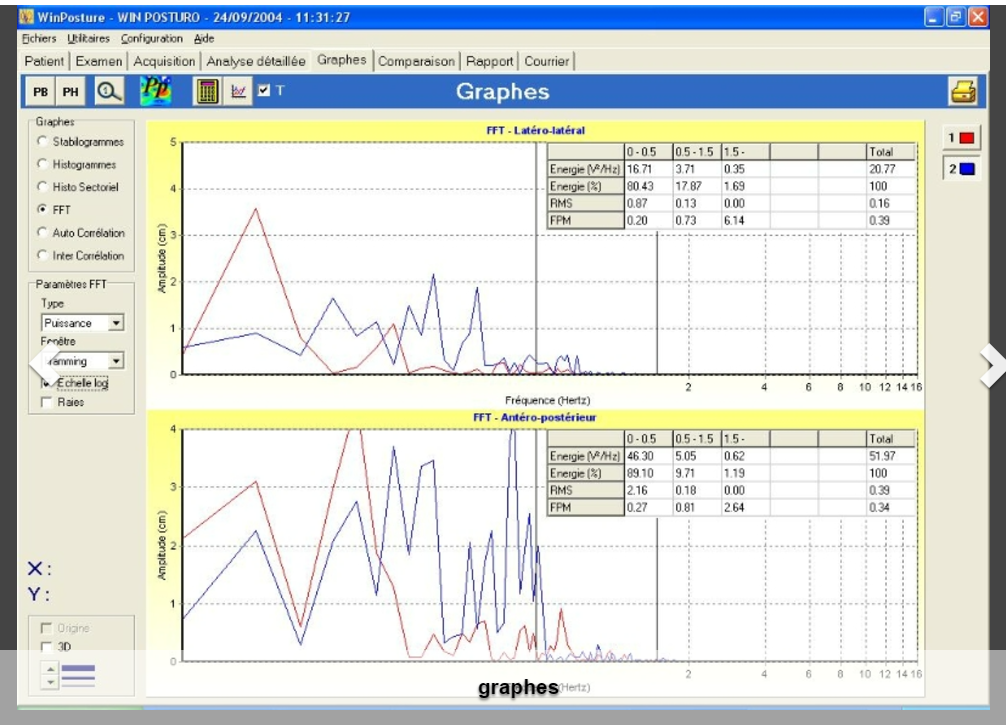
\includegraphics[height=5cm]{images/pression_plantaire/winposture2.png}
    \caption{Logiciel de visualisation Winposture}\label{fig: Logiciel Winposture}
    \end{subfigure}\\
    \begin{subfigure}[b]{0.45\textwidth}
      \centering
      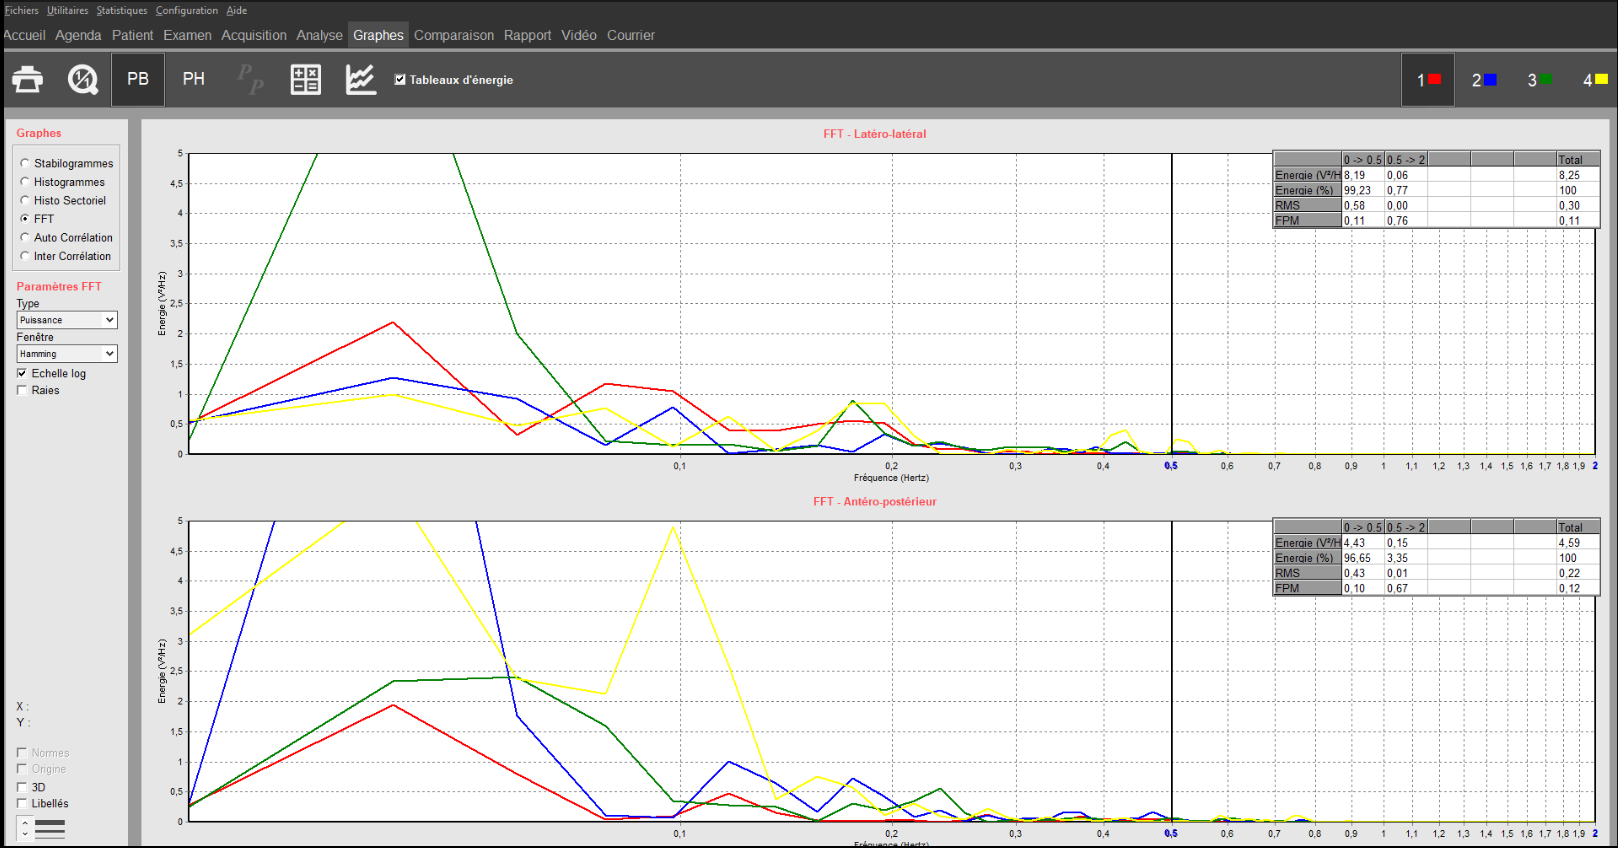
\includegraphics[height=4cm]{images/analyse_marche/FFT.png}
      \caption{Fenêtres d’analyse fréquentielle Fusyo (FFT)}\label{fig:FFT}
    \end{subfigure}
    \begin{subfigure}[b]{0.45\textwidth}
      \centering
      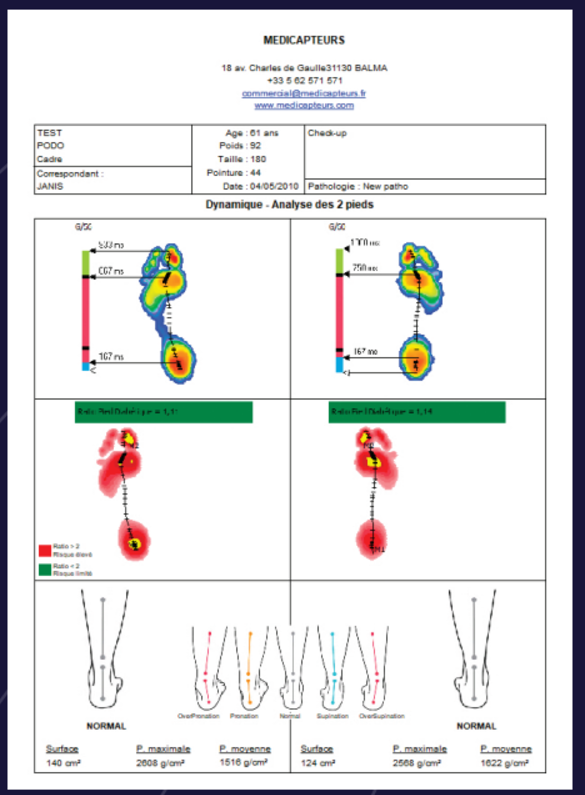
\includegraphics[height=5cm]{images/analyse_marche/WinPod4.png}
    \caption{Les rapports générés personnalisable Win-pod}\label{fig:WinPod4}
    \end{subfigure}
    \caption{Rapports générés personnalisables Win-pod}\label{fig:global2}
  \end{figure}

\newpage
\section{Stratégie de développement}


\subsection{Analyse du marché}

Cette analyse de marché a pour objectif de présenter les différentes 
plateformes d'analyse de stabilométrie, en mettant en avant leurs spécificités et 
fonctionnalités, afin d’identifier et répondre aux besoins des professionnels de 
santé. 
La plupart de ces plateformes de visualisation se distinguent par leur 
convivialité et leur ergonomie, facilitant leur utilisation (Figure 5(a)).  
Elles offrent la possibilité de créer et de gérer des protocoles d’acquisition 
tout en permettant de paramétrer des normes conformes aux plateformes 
stabilométriques utilisées. Ces logiciels intègrent des fonctionnalités avancées 
telles que l’analyse fréquentielle et l’analyse temporelle (Figure 5(b)). Elles 
permettent également de comparer les résultats des examens pour chaque patient, 
avec des données facilement exportables. Les rapports et bilans générés sont 
entièrement personnalisables ce qui permet au médecin de garder un bilan détaillé 
du premier examen patient (Figure 5(c)).

\begin{figure}[H]
    \centering
    \begin{subfigure}[b]{0.45\textwidth}
      \centering
      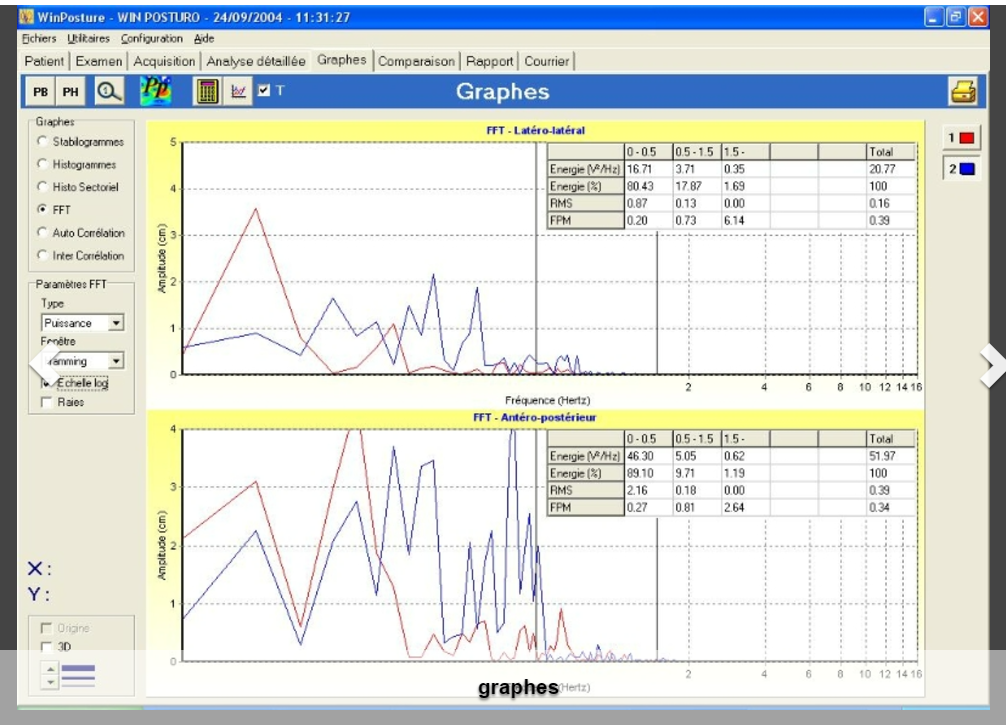
\includegraphics[height=5cm]{images/pression_plantaire/winposture2.png}
    \caption{Logiciel de visualisation Winposture}\label{fig: Logiciel Winposture}
    \end{subfigure}\\
    \begin{subfigure}[b]{0.45\textwidth}
      \centering
      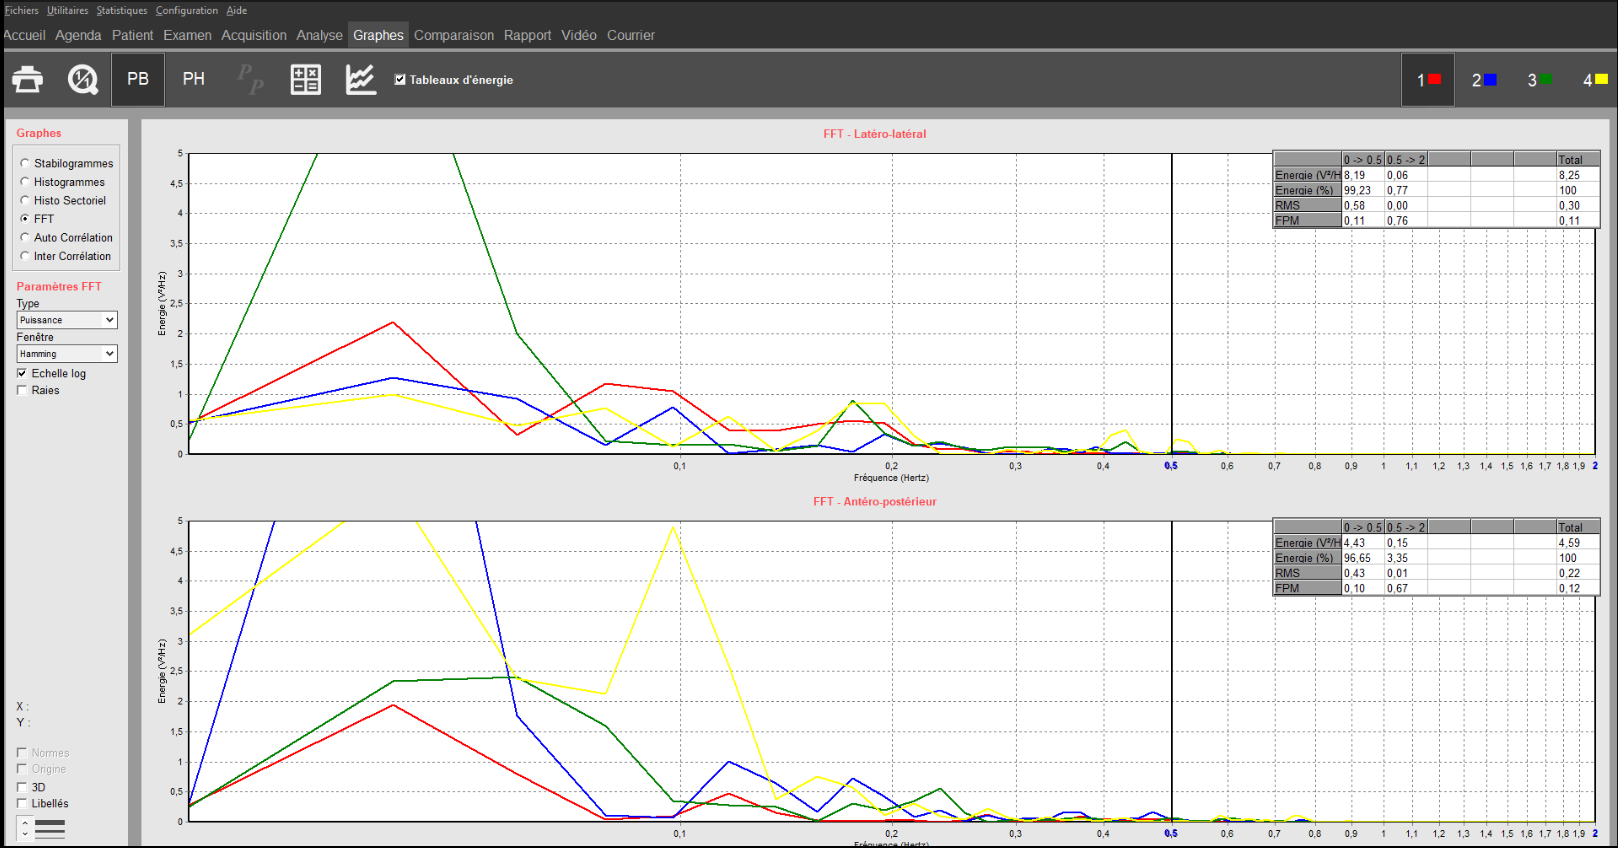
\includegraphics[height=4cm]{images/analyse_marche/FFT.png}
      \caption{Fenêtres d’analyse fréquentielle Fusyo (FFT)}\label{fig:FFT}
    \end{subfigure}
    \begin{subfigure}[b]{0.45\textwidth}
      \centering
      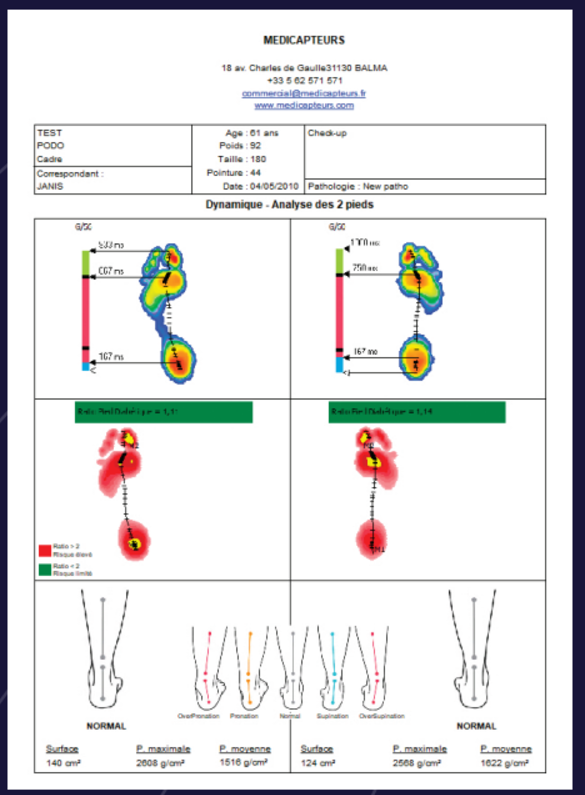
\includegraphics[height=5cm]{images/analyse_marche/WinPod4.png}
    \caption{Les rapports générés personnalisable Win-pod}\label{fig:WinPod4}
    \end{subfigure}
    \caption{Rapports générés personnalisables Win-pod}\label{fig:global2}
  \end{figure}
\subsection{Conception}

\subsubsection{Fonctionnalités intégrées}
Lors de la phase de développement, l'accent sera mis sur une production d'interface graphique simple, ergonomique et intuitive.
Le but est de fournir une application qui puisse être utilisée sans formation préalable, avec une installation la plus simple possible, sans sacrifier de fonctionnalité.

Afin de faciliter le développement de la plateforme de visualisation, cette dernière sera séparée en deux parties, comme les conventions de développement actuelles l'entendent. 
La partie dite \textbf{serveure} (backend) sera chargée des calcul et du rassemblement d'information. 
La partie dite \textbf{cliente} (frontend) sera, quant à elle, chargée de l'affichage des résultats.

Les utilisateurs verront uniquement la partie frontend, et selon les entrées spécifiés (les différents paramètres que les utilisateurs spécifieront), le frontend communiquera avec la partie backend pour que cette dernière effectue les calculs demandés, ou réunisse les informations nécessaires et les lui retourne.

\subsubsection{Ressources utilisées}

\textbf{Partie serveur} \\
Le langage envisagé pour la partie serveure est le Python.
Ce langage existe depuis 1991, et a été très largement adopté dans les communautés scientifiques.
Python bénéficie aujourd'hui d'un nombre impressionnant de librairies qui seront extrêmement pratiques pour la manipulation des données, les calculs ainsi que les rendus graphiques.
Pour créer le serveur qui permettra la connexion à une base de données ou les calculs divers, plusieurs choix sont possibles.
Django est un framework python largement utilisé dans tous les domaines.

En tant qu'alternative, la partie serveure pourrait aussi être développée en Ruby, un autre langage très utilisé pour les serveurs.
Le framework utilisé dans ce cas là serait Ruby on Rails.

\textbf{Partie cliente} \\
Pour la partie cliente, le développement se fera avec NextJS ainsi qu'avec NodeJS.
NextJS est un langage basé sur le TypeScript qui permet un grand contrôle sur la création d'interface et son comportement.
C'est un framework moderne, reconnu pour sa sécurité et largement adopté par des multinationales.
NodeJS est un framework JavaScript permettant de gérer des modules à ajouter à l'application (ici par exemple, les modules permettant la visualisation des graphiques, les modules de communications avec le backend, et d'autres).

\textbf{Base de données} \\
En termes de base de données pour le stockage des informations patients, il est judicieux d’opter pour une base de données locale (qui ne sera pas hébergée en ligne) écrite en SQLite.
Ce langage permet de créer des bases de données légère et rapides.
SQLite a été largement adopté pour tout type d’application nécessitant une base de données locale.

\subsubsection{Prototype}
La plateforme de visualisation des signaux posturographique imaginée à été conçue 
pour être intuitive, simple d’utilisation ainsi que ergonomique facilitant au 
quotidien le diagnostic du médecin. Dès la page d’accueil, ce dernier peut accéder 
à l’ensemble de ses dossiers patients afin d’assurer un suivi personnalisé 
(Figure 6(a)). La plateforme permet également de visualiser les données 
enregistrées par la plateforme stabilométrique 
De plus, il est possible de visualiser les données 
(enregistrées par la plateforme stabilométrique) dans les domaines fréquentiels 
et temporels, tout en offrant la possibilité de sélectionner différents protocoles 
expérimentaux afin de comparer les résultats obtenus (Figure 6(b)). Le médecin a 
la possibilité d’ajuster différents paramètres, tels que la fréquence 
d’échantillonnage ou la durée d’observation des relevés de données.  Il dispose 
aussi d’un accès à des données synthétiques clés, comme la moyenne, la médiane ou 
l’écart-type, pour une analyse rapide (Figure 6(c)). Par ailleurs, la plateforme 
permet d’évaluer la stabilité du patient à travers divers examens cliniques, 
favorisant une corrélation entre les résultats cliniques et les données 
enregistrées. Enfin, chaque observation peut être exportée au format PDF à la fin 
de l’analyse, incluant les commentaires du médecin pour conserver une trace des 
conclusions tirées lors de l’étude.

\begin{figure}[H]
    \centering
    \begin{subfigure}[b]{0.45\textwidth}
      \hspace*{-2cm}
      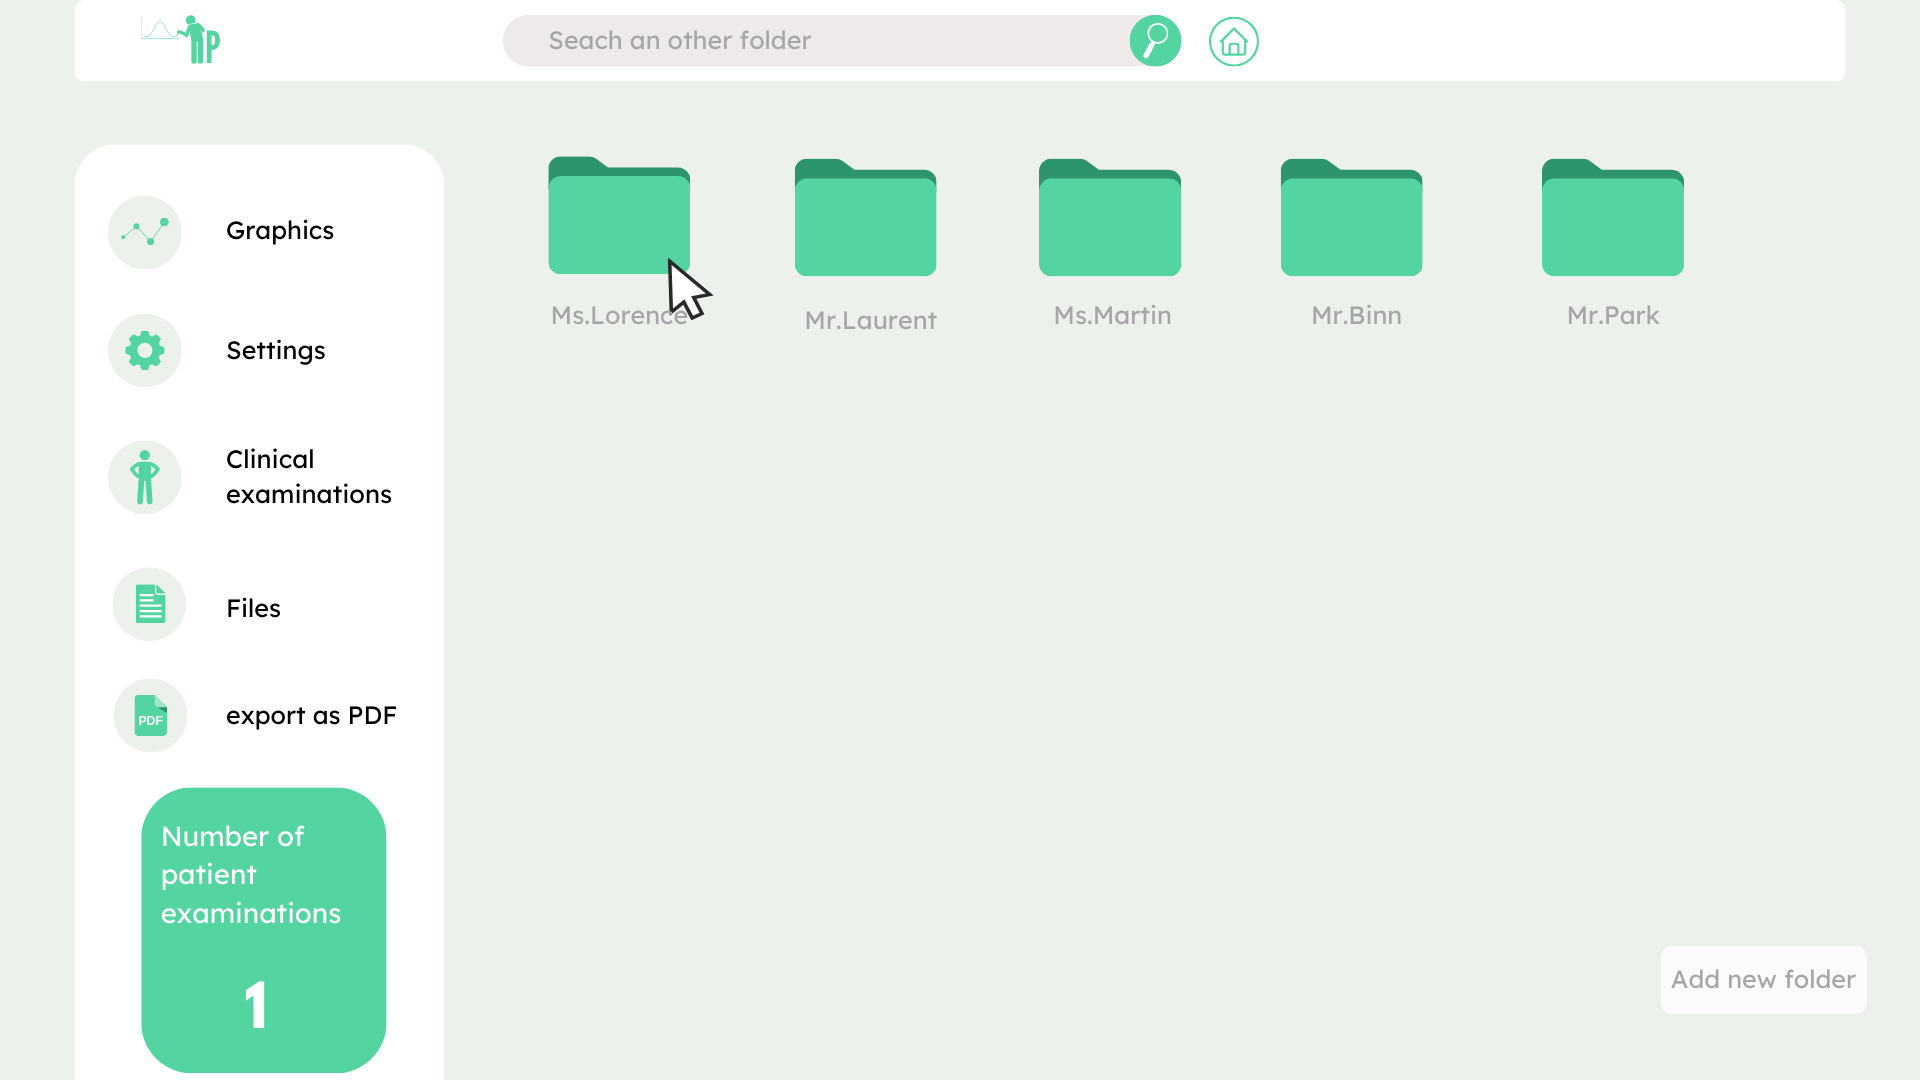
\includegraphics[height=5cm]{images/Prototype/Accueil de la plateforme de visualisation.png}
      \caption{Accueil de la plateforme de visualisation}\label{fig:Accueil de la plateforme de visualisation}
    \end{subfigure}
    \begin{subfigure}[b]{0.45\textwidth}
        \centering
      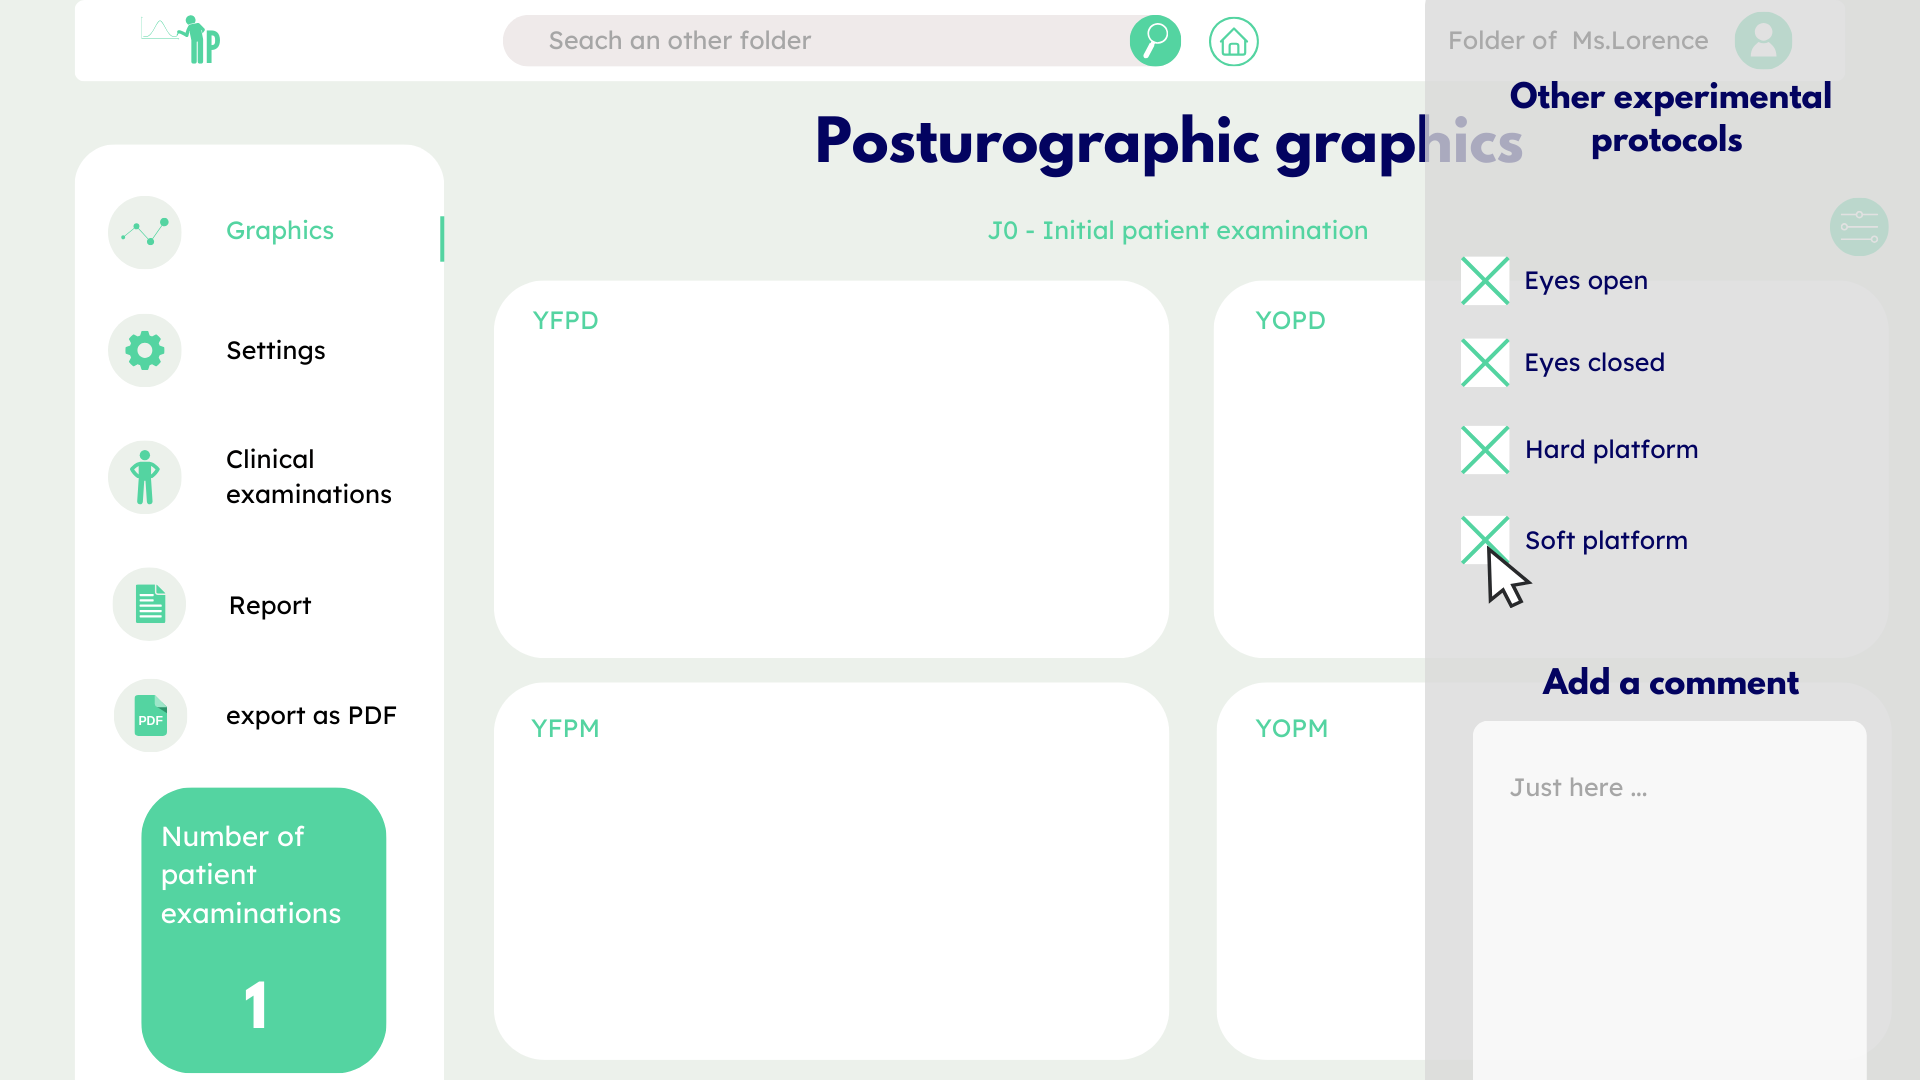
\includegraphics[height=5cm]{images/Prototype/Visualisation des données en fonction de différents protocoles expérimentaux.png}
      \caption{Visualisation des données en fonction de différents protocoles expérimentaux}\label{fig:Visualisation des données en fonction de différents protocoles expérimentaux}
    \end{subfigure}\\
    \begin{subfigure}[b]{0.45\textwidth}
      \centering
      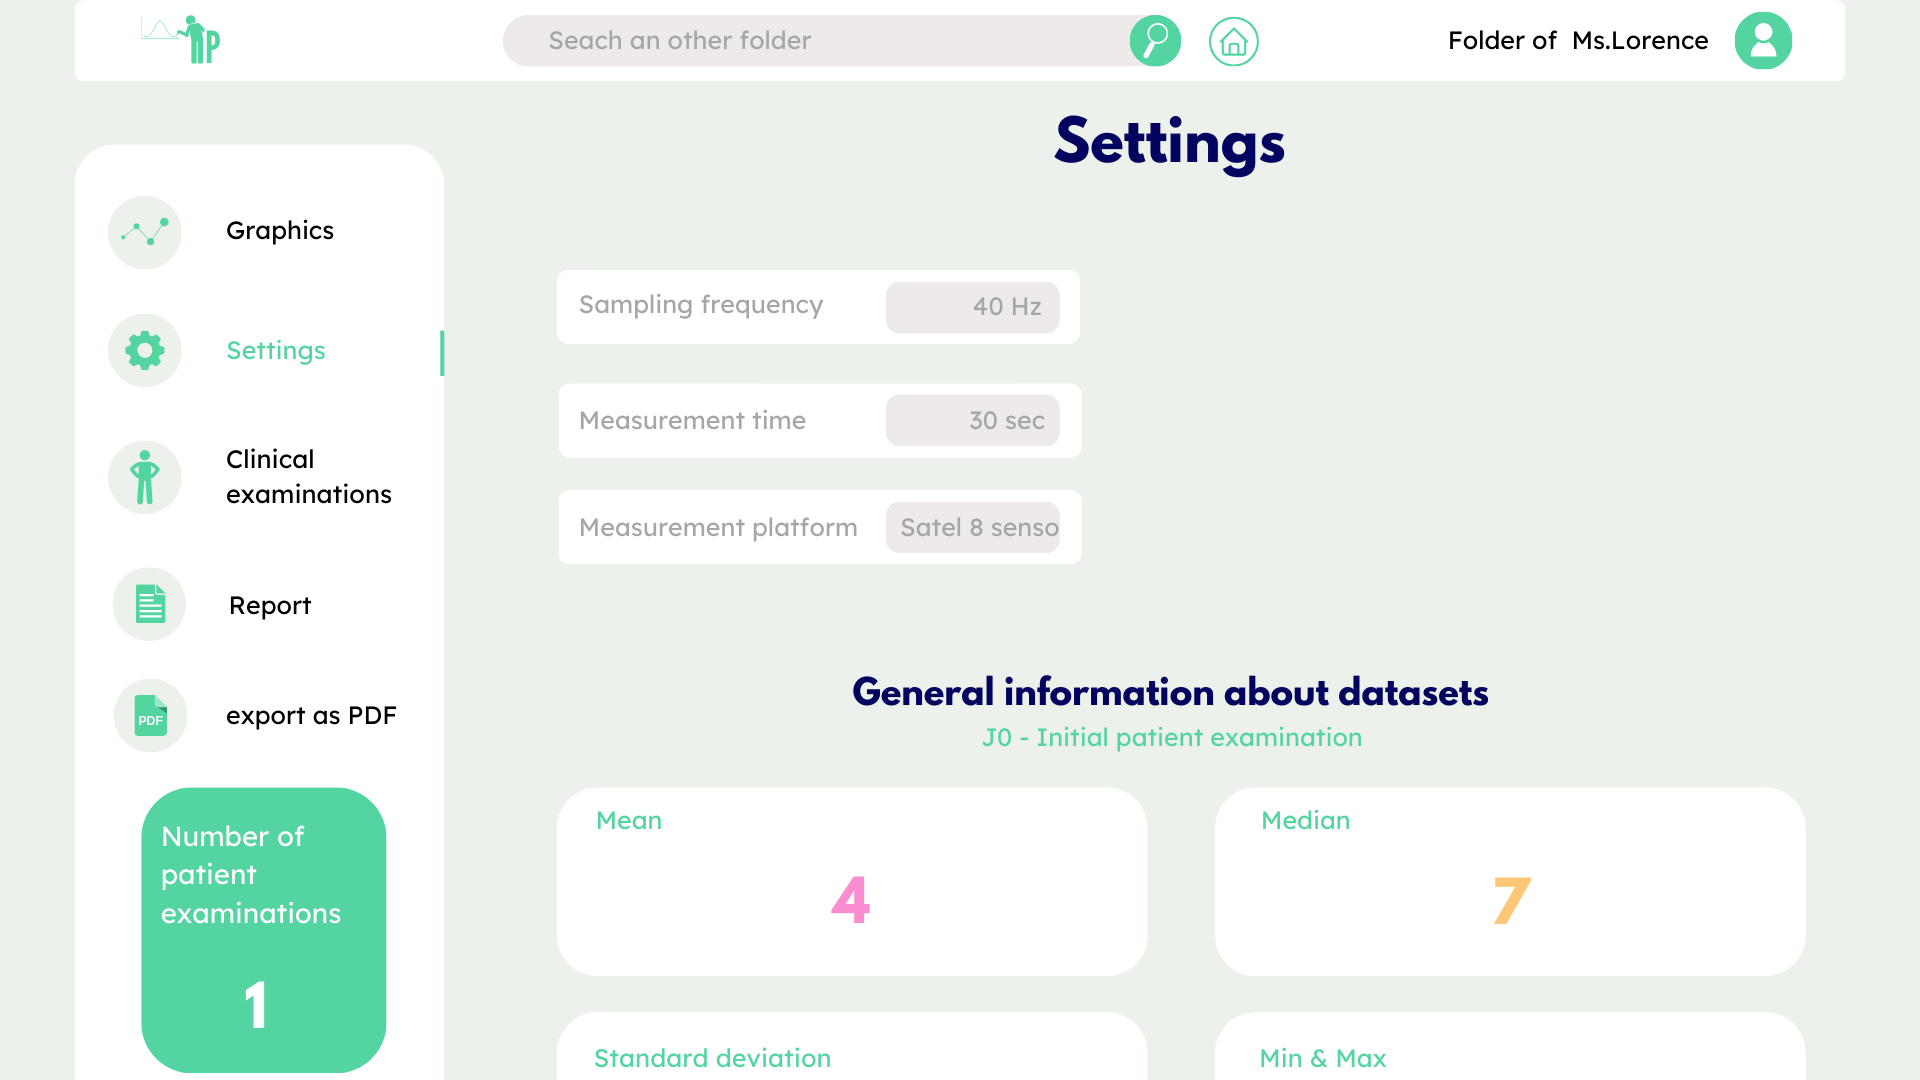
\includegraphics[height=5cm]{images/Prototype/visualiser des données clés du jeu de données étudié.png}
    \caption{visualiser des données clés du jeu de données étudié }\label{fig:visualiser des données clés du jeu de données étudié }
    \end{subfigure}
    \caption{Plateforme de posturographie imaginée}\label{fig:globalposturographie}
  \end{figure}


\newpage
\section{Gestion de projet}

\subsection{Phase de développement}
\subsection{Outils utilisés}

\newpage
\section{Conclusion}

La création d'une plateforme posturographique est non négligeable lorsque  l'analyse des signaux posturagraphique joue un rôle aussi essentiel dans le diagnostic médical et le suivi des patients. Face à la complexité des données reçues à l’issue des examens posturographiques, il est primordial de proposer un outil simplifiant cette analyse, tout en permettant aux médecins de gagner en efficacité et en précision. L'objectif est ainsi de rendre les résultats plus accessibles, compréhensibles et exploitables rapidement.
Au cours des quatre semaines de travail,  plusieurs étapes ont été essentielles pour concrétiser ce projet. Tout d'abord, des recherches approfondies ont été menées sur la posturographie, en particulier la posturographie statique, afin de comprendre les principes de mesure et les signaux générés par les différentes techniques. Cette étape a permis de définir clairement les besoins et les fonctionnalités attendues. Ensuite, nous avons imaginé une première version de la plateforme en élaborant une structure fonctionnelle capable de répondre aux exigences d'analyse et d'utilisation.
Les résultats obtenus jusqu'à présent témoignent d'une avancée significative dans la conceptualisation de la plateforme. Une compréhension approfondie des signaux posturographiques et des besoins des médecins a été acquise, posant ainsi des bases solides pour le développement futur.
Au cours du deuxième semestre, nous prévoyons d'orienter nos efforts vers le développement technique de la plateforme en veillant à son ergonomie ainsi que sa performance. L'objectif sera de livrer un outil fonctionnel, adapté aux besoins des médecins, capable d'offrir une analyse rapide, précise et intuitive des signaux posturographiques. Ce travail contribuera à améliorer l'efficacité des évaluations posturales et à faciliter la prise de décisions médicales.

\end{document}
